\documentclass{report}
\usepackage{draftwatermark}
\SetWatermarkText{DRAFT}
\SetWatermarkScale{7}
\title{Radio Collar Tracker Flight Operations Manual}
\author{Eric Lo, Project Manager\\Nathan Hui, Project Lead\\Engineers for Exploration, UC San Diego}
\usepackage{fullpage}
\usepackage{hyperref}
\usepackage{mdframed}
\usepackage{bookmark}
\usepackage[toc]{glossaries}
\makeglossaries
\hypersetup{
    colorlinks,
    citecolor=black,
    filecolor=black,
    linkcolor=black,
    urlcolor=blue
}

% Glossaries Definition
\newacronym{uas}{UAS}{Unmanned Aerial System}
\newacronym{gcs}{GCS}{Ground Control System}
\newacronym{pic}{PIC}{Pilot In Command}
\newglossaryentry{multirotor}{
	name=multirotor,
	description={is an unammed aircraft with multiple propellers for lift},
	plural=multirotors
}
\newglossaryentry{quadcopter}{
	name=quadcopter,
	description={is a multirotor with 4 propellers},
	plural=quadcopters
}
\newglossaryentry{LiPo}{
	name=LiPo,
	description={is a battery using a lithium polymer chemistry},
	plural=LiPos
}
\newglossaryentry{sdr_gls}{
	name={software defined radio},
	description={is a radio that uses software instead of hardware to process and interpret the signal}
	plural={software defined radios}
}
\newacronym[see={[Glossary:]{sdr_gls}}]{SDR}{SDR}{\gls{sdr_gls}}
\newacronym{rtl}{RTL}{Return To Launch}
\newacronym{AO}{AO}{Autopilot Operator}

\begin{document}
\maketitle
\tableofcontents
\chapter{Manual Objective}
	This manual is intended for the end user of the Radio Collar Tracker system.  It is written with the expectation that the end user has some experience flying \glspl{multirotor} in semi-autonomous or autonomous modes.  This manual should not be regarded as standalone training manual for flight operations, rather, it should part of hands-on training on how to operate this system safely.  This manual contains procedures on how to safely operate this system, as well as information on how to maintain and repair the system.
\chapter{System Overview}
	\section{Mission Profile}
		This system is designed to conduct aerial surveys for the purpose of tracking and localizing wildlife collars used for biological and ecological research.  We approach this problem by flying a radio across the search area, recording the signal strength for any pings from any collars we can detect.  We can then determine the location of a collar by correlating the signal strength and the locations where we detected that particular signal strength.
	\section{Aircraft}
		\subsection{Aircraft Summary}
			The airframe used in this \gls{uas} is a Tarot Ironman 650, which is a carbon-fiber \gls{quadcopter} airframe.  We have then integrated a commercial open-source autopilot, the 3DR PixHawk, to use as our primary flight controller.  To maximize flight time, we have settled on a battery pack consisting of 3 3S 5.1 Ah batteries connected in parallel.  As a result of this configuration, we can acheive a total flight time of 20-23 minutes at a maximum speed of 5 m/s.
		\subsection{Aircraft Specifications}
			\begin{itemize}
				\item Length\hfill110 cm
				\item Width\hfill89 cm
				\item Height\hfill25 cm
				\item Empty Weight\hfill1.5 kg
				\item Maximum Takeoff Weight\hfill
				\item Diagonal Boom Length\hfill65 cm
				\item Powerplant\hfill 4 x Navigator Series T-Motor MN4010-11
				\item Powerplant kV Rating\hfill475
				\item Powerplant Voltage\hfill12.5 V
				\item Maximum Speed\hfill 5 m/s
				\item Maximum Range\hfill 6 km
				\item Rotor Diameter\hfill 43 cm
				\item Rotors\hfill4
				\item Battery\hfill 3S 3P 24C \gls{LiPo} 15300 mAh
				\item Battery Weight\hfill 1 kg
				\item Autopilot\hfill3DR Pixhawk
				\item RC Receiver\hfill FrSky X8R
				\item Autopilot Datalink Radio\hfill 3DR 915 MHz Radio
				\item Motor Controller\hfill 4 x HobbyKing Platinum Pro 30A
				\item Base Airframe\hfill Tarot Ironman 650 TI65B01
				\item RC Transmitter\hfill FrSky Taranis X9D
			\end{itemize}
		\subsection{Transmitter Layout}
			\begin{figure}[ht]
				\centering
				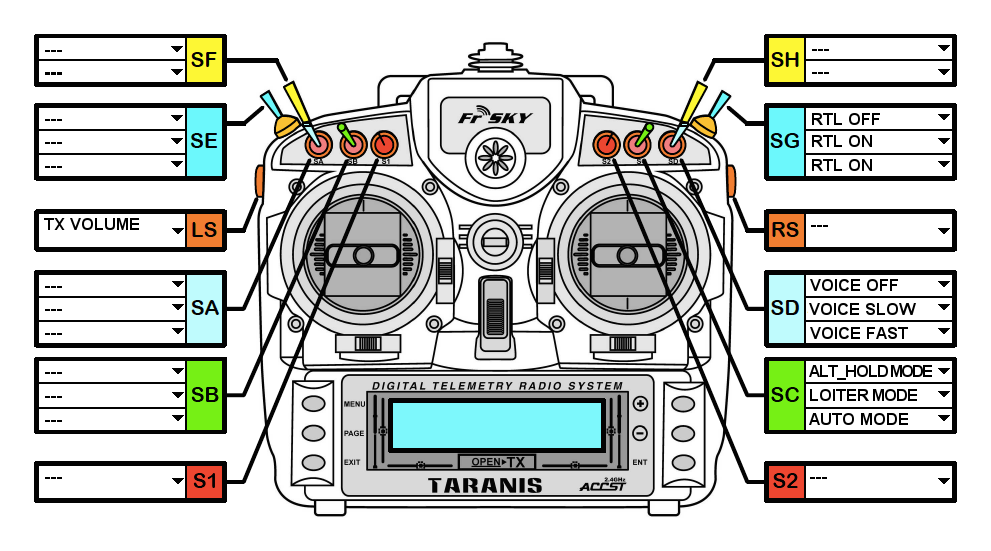
\includegraphics[width=\textwidth]{taranis_layout.png}
				\caption{FrSky Taranis X9D Switch Assignments}
			\end{figure}
			\subsubsection{Flight Modes}
				This \gls{uas} has multiple flight modes that allow the \gls{pic} various amounts of control, and permit the \gls{uas} to perform a variety of tasks.  These flight modes are all to some extent controlled by the computer, and can be controlled from either the RC transmitter or the \gls{gcs}.
				\paragraph{Stabilize}
					Stabilize (shown as STABILIZE) is the most basic mode available.  In this mode, the \gls{pic} has direct control over the attidue and throttle of the aircraft. See Figure 2.2 for stick layout.
					\begin{figure}[ht]
						\centering
						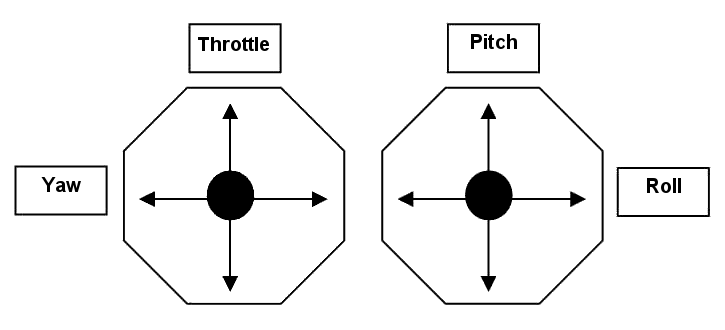
\includegraphics[width=0.5\textwidth]{stabilize_stick_layout.png}
						\caption{Stabilize Stick Layout}
					\end{figure}
				\paragraph{Altitude Hold}
					Altitude Hold (shown as ALT\_HOLD) is one step above STABILIZE in computer control.  In this mode, the \gls{pic} has direct control over the attidue of the aircraft, however, the autopilot is responsible for maintaining the altitude of the aircraft.  Because the autopilot is actively controlling the aircraft, this is a GPS-controlled mode, and requires optimal GPS lock.  Altitude is held by placing the throttle stick to 50\%.  Pushing the throttle stick up moves the altitude setpoint up at a rate proportional to the stick value, and vice versa.  See Figure 2.3 for stick layout.
					\begin{figure}[ht]
						\centering
						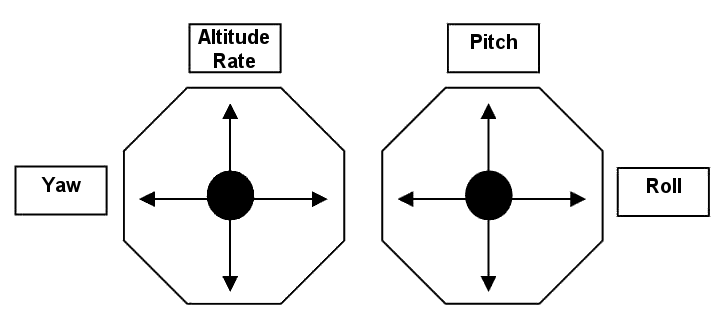
\includegraphics[width=0.5\textwidth]{althold_stick_layout.png}
						\caption{Altitude Hold Stick Layout}
					\end{figure}
				\paragraph{Loiter}
					Loiter (shown as LOITER) is one step below complete computer control.  In this mode, the \gls{pic} can only tell the aircraft to move.  The autopilot is responsible for maintaining the altitude, attitude, and responsiveness of the aircraft.  Essentially, the aircraft is simply loitering at a point in space, and the \gls{pic} is simply telling the aircraft that it should go loiter somewhere else.  Because the autopilot is actively controlling the aircraft, this is a GPS-controlled mode, and requires optimal GPS lock.  Altitude is held by placing the throttle stick to 50\%.  Pushing the throttle stick up moves the altitude setpoint up at a rate proportional to the stick value, and vice versa.  See Figure 2.4 for stick layout.
					\begin{figure}[ht]
						\centering
						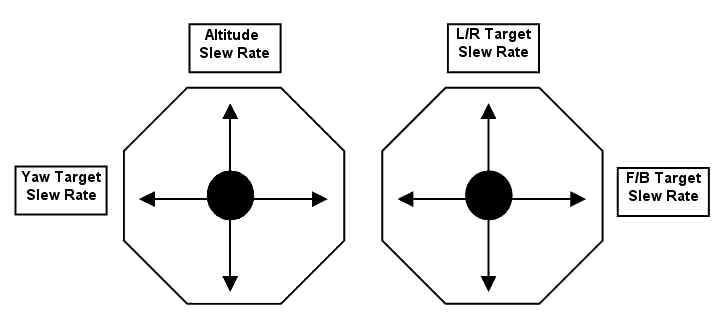
\includegraphics[width=0.5\textwidth]{loiter_stick_layout.png}
						\caption{Loiter Stick Layout}
					\end{figure}
				\paragraph{Auto}
					Auto (shown as AUTO) is the autonomous mission mode.  In this mode, the autopilot has complete control authority over the aircraft.  The \gls{pic} can only command the \gls{uas} to enter or exit this mode.  The autopilot will execute the loaded mission, controlled from the \gls{gcs}.  Because the autopilot is actively controlling the aircraft, this is a GPS-controlled mode, and requires optimal GPS lock.
				\paragraph{Return-to-Launch}
					\gls{rtl} is an emergency retrieval mode.  In this mode, the autopilot has complete control authority over the aircraft.  The \gls{pic} can only command the \gls{uas} to enter or exit this mode.  The autopilot will command the aircraft to fly directly to the launch GPS coordinates, then gently land.  Because the autopilot is actively controlling the aircraft, this is a GPS-controlled mode, and requires optimal GPS lock.  During the landing phase, the \gls{pic} can nudge the aircraft using the right stick to avoid any obstacles.  This is similar to loiter, however, the \gls{pic} cannot override the descent phase without exiting the \gls{rtl} mode.  See Figure 2.5 for stick layout.
					\begin{figure}[ht]
						\centering
						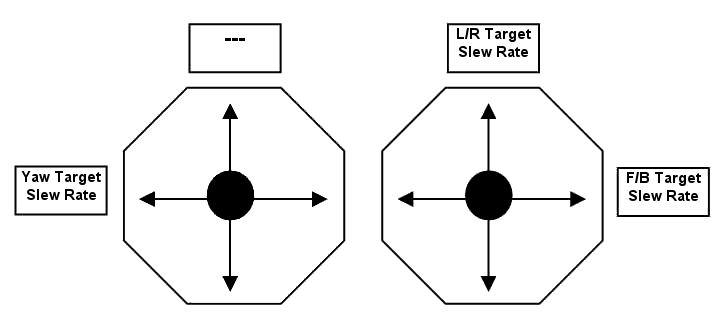
\includegraphics[width=0.5\textwidth]{rtl_stick_layout.png}
						\caption{RTL Stick Layout}
					\end{figure}
		\subsection{Aircraft Layout}
	\section{Payload}
		\subsection{Payload Summary}
			The payload for this \gls{uas} is basically a computerized radio recorder.  We have elected to use a software defined radio as our radio frontend, as this allows us to rapidly reconfigure the payload for any range of frequencies.  This is connected to a Raspberry PI 2, which handles all of the data collection, including collecting position data from the autopilot system.  Recorded data is organized into runs, which are stored on a removeable USB drive.
		\subsection{Payload Specifications}
			\begin{itemize}
				\item Computer\hfill Raspberry Pi 2
				\item Weight \hfill 125 g
			\end{itemize}
		\subsection{Payload Layout}
			See Figure 2.6.
			\begin{figure}[ht]
				\centering
				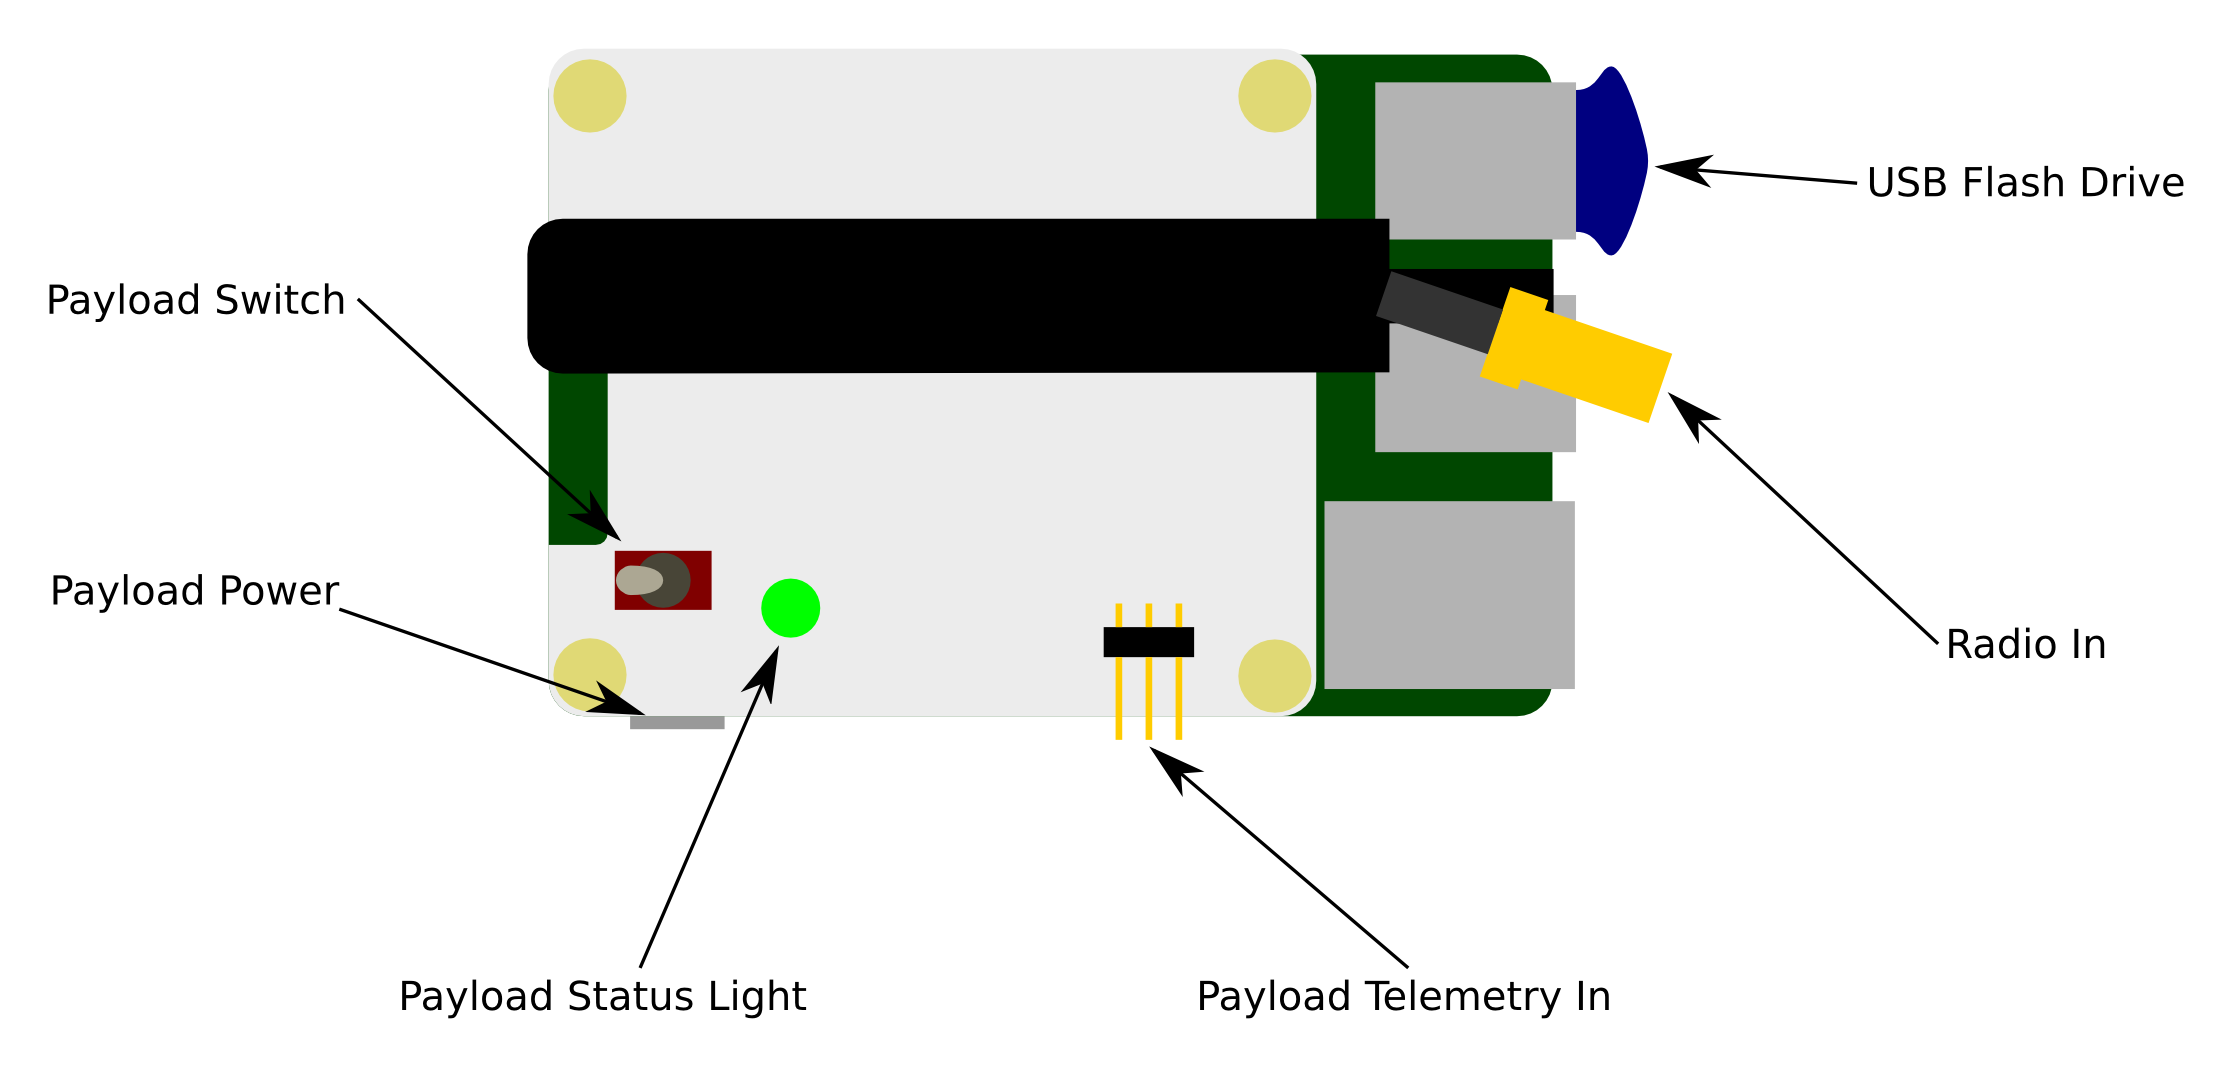
\includegraphics[width=\textwidth]{payload_layout.png}
				\caption{Payload Layout}
			\end{figure}
	\section{Ground Control System}
		The \gls{gcs} for this \gls{uas} consists of a laptop running a Windows OS and the open source flight management software, MissionPlanner.  This connects to the aircraft over a 3DR 900 MHz radio, permitting 2-way digital communications between the \gls{uas} and the \gls{gcs}.  From the \gls{gcs}, we are able to plan, upload, and control all missions, as well as provide the pilot with flight and diagnostic information.
		\subsection{Ground Control System Layout}
	\section{Crew Roles}
		\subsection{Pilot In Command}
			The \gls{pic} is responsible for the safe operation of the aircraft.  He or she is responsible for takeoff, transition to mission, return, and landing, as well as for the general pacing of the mission.
		\subsection{Autopilot Operator}
			The \gls{AO} is responsible for monitoring the flight management software and mission progress.  He or she must plan and upload the mission plan to the aircraft, confirm clearance for switching to autonomous flight modes, and monitor the \gls{uas} as it completes the mission.
\chapter{Checklists and Flight Procedures}
	The \gls{pic} must use the below checklists and procedures when operating the system to ensure safe and proper operation of the system.  Failure to complete all items in either checklists or procedures may result in system misconfiguration or system failure.  The PIC is responsible for the operation of the aircraft in accordance with all relevant rules and procedures, except that the PIC may deviate from these rules where such deviation is necessary in the interests of safety.
	\section{Battery Cold Swap Procedure}
		\begin{enumerate}
			\item Disconnect BATTERY PARALLEL ADAPTER from AIRCRAFT POWER.
			\item Disconnect BATTERY PARALLEL ADAPTER from PAYLOAD POWER.
			\item Remove the old AIRCRAFT BATTERY.
			\item Attach the new AIRCRAFT BATTERY to the BATTERY BOOMS.
			\item Connect the BATTERY PARALLEL ADAPTER to the AIRCRAFT BATTERY.
			\item Check the AIRCRAFT CENTER OF GRAVITY.
		\end{enumerate}
	\section{Before Aircraft and Payload Power On Check}
		\begin{enumerate}
			\item AIRCRAFT POWER \hrulefill DISCONNECTED
			\item AIRCRAFT BATTERIES \hrulefill 4.18 V $\pm$ 0.01 V PER CELL, MATCHED PACKS
			\item AIRCRAFT CENTER OF GRAVITY \hrulefill CHECK
			\item AIRCRAFT ROTOR ALIGNMENT \hrulefill CHECK
			\item AIRCRAFT ROTOR INTEGRITY \hrulefill CHECK
			\item AIRCRAFT BOOM INTEGRITY \hrulefill CHECK
			\item AIRCRAFT BATTERY STRAPS \hrulefill SECURED
			\item BATTERY PARALLEL ADAPTER \hrulefill ATTACHED TO BATTERIES
			\item PAYLOAD POWER \hrulefill DISCONNECTED
			\item PAYLOAD SWITCH \hrulefill OFF
			\item PAYLOAD ANTENNA \hrulefill CHECK
			\item MAVLINK \hrulefill DISCONNECTED
			\item \gls{gcs} DATALINK \hrulefill ACTIVE AND CONFIGURED
			\item RC TRANSMITTER \hrulefill ACTIVE
			\begin{enumerate}
				\item MODE SWITCH \hrulefill STABILIZE
				\item RIGHT STICK \hrulefill CENTERED/DOWN
				\item LEFT STICK \hrulefill CENTERED
				\item TRIMS (ALL) \hrulefill CENTERED
				\item AUTO SWITCH \hrulefill OFF
				\item \gls{rtl} SWITCH \hrulefill OFF
			\end{enumerate}
		\end{enumerate}
	\section{Aircraft and Payload Power On Procedure}
		\begin{enumerate}
			\item Connect PAYLOAD POWER.
			\item Connect AUTOPILOT POWER.
			\item Do not rock the aircraft.
			\item Verify PAYLOAD STATUS LIGHT is flashing slowly within 15 seconds.
			\item Verify AUTOPILOT STATUS LIGHT is flashing slowly within 30 seconds.
			\item Connect the \gls{gcs} MAVLINK.
		\end{enumerate}
	\section{Pre-Takeoff Check}
		\begin{enumerate}
			\item GPS STATUS \hrulefill AT LEAST 6
			\item GPS LOCATION \hrulefill STABLE, REASONABLE
			\item ORIENTATION \hrulefill HORIZONTAL
			\item AIRSPACE \hrulefill CLEAR
			\item TAKEOFF CLEARANCE \hrulefill CLEAR
			\item AUTOPILOT OPERATOR \hrulefill NOTIFIED
			\item PAYLOAD SWITCH \hrulefill ON
		\end{enumerate}
	\section{Paylaod Start Procedure}
		% TODO
	\section{Takeoff Procedure}
		\begin{enumerate}
			\item Set the RC TRANSMITTER MODE SWITCH to LOITER.
			\item Set THROTTLE to 0\%.
			\item Disengage aircraft safeties by pressing and holding the AIRCRAFT SAFETY SWITCH.
			\item Confirm that the AIRCRAFT SAFETY SWITCH is solid red.
			\item Arm the THROTTLE ARM by holding the left stick down and to the right.
			\item Advance THROTTLE to 50\%.
			\item Add takeoff power.
			\item Reduce THROTTLE when approaching hover altitude.
		\end{enumerate}
	\section{Sub-optimal Takeoff Procedure}
		\begin{enumerate}
			\item Set the RC TRANSMITTER MODE SWITCH to STABILIZE.
			\item Set THROTTLE to 0\%.
			\item Disengage aircraft safeties by pressing and holding the AIRCRAFT SAFETY SWITCH.
			\item Confirm that the AIRCRAFT SAFETY SWITCH is solid red.
			\item Arm the THROTTLE ARM by holding the left stick down and to the right.
			\item Advance THROTTLE to 15\%.
			\item Check for control authority.
			\item Add takeoff power.
			\item Manuever to clear obstacles, until adequate clearance and/or GPS stability.
			\item Reduce THROTTLE when approaching hover altitude.
		\end{enumerate}
	\section{Climb to Hover in LOITER or ALT\_HOLD Procedure}
		\begin{enumerate}
			\item Add power to climb.
			\item Reduce THROTTLE to 50\% when approaching hover altitude.
			\item Check with \gls{gcs} for status.
		\end{enumerate}
	\section{Climb to Hover in STABILIZE Procedure}
		\begin{enumerate}
			\item Add power to climb.
			\item Reduce THROTTLE when approaching hover altitude.  Adjust to maintain altitude.
			\item Check with \gls{gcs} for status.
		\end{enumerate}
	\section{Pre-Mission Start Check}
		\begin{enumerate}
			\item LOITER CLEARANCE\hrulefill CHECK
			\item MISSION\hrulefill UPLOADED
			\item WINDS\hrulefill LESS THAN 8 M/S
		\end{enumerate}
	\section{Mission Start Procedure}
		\begin{enumerate}
			\item Set the RC TRANSMITTER MODE SWITCH to LOITER.
			\item Confirm with \gls{gcs} that LOITER mode is set and stable.
			\item Notify \gls{gcs} of intent to enter AUTO mode.
			\item Set the RC TRANSMITTER MODE SWITCH to AUTO.
			\item Confirm switch to WAYPOINT with \gls{gcs}.
		\end{enumerate}
	\section{Mission End Procedure}
		\begin{enumerate}
			\item Check that the RC TRANSMITTER is on and active.
			\item Check that the aircraft is within visual range.
			\item Check that there is enough battery to land safely.
			\item Notify \gls{gcs} of intent to take control of the aircraft.
			\item Set the RC TRANSMITTER MODE SWITCH to LOITER.
			\item Confirm with \gls{gcs} that the pilot has control of the aircraft.
		\end{enumerate}
	\section{Failed Mission End Procedure}
		\begin{enumerate}
			\item Set the RC TRANSMITTER MODE SWITCH to AUTO.
			\item Notify \gls{gcs} of failure to take control of the aircraft.
			\item Have \gls{gcs} set the RETURN TO HOME mode.
			\item Continuously retry the MISSION END PROCEDURE until control is regained.
			\item If control cannot be regained, but the aircraft is in RETURN TO HOME mode, allow the aircraft to autonomously land.
			\item If control cannot be regained, and the aircraft is not in RETURN TO HOME mode, execute the LOSS OF AUTOPILOT DATALINK procedure.
		\end{enumerate}
	\section{Pre-Approach Checks}
		\begin{enumerate}
			\item APPROACH \hrulefill CLEAR
			\item TRAFFIC \hrulefill CLEAR
			\item RC TRANSMITTER MODE SWITCH \hrulefill LOITER
		\end{enumerate}
	\section{Approach Procedure}
		\begin{enumerate}
			\item Reduce THROTTLE to begin descent.
			\item Fly the approach at a non-vertical angle, with a descent rate no greater than 2 m/s
			\item Enter a hover at 2-5 meters AGL above the landing area.
		\end{enumerate}
	\section{Landing Procedure}
		\begin{enumerate}
			\item Reduce THROTTLE to enter a controlled vertical descent, with a descent rate no greater than 2 m/s.
			\item When the aircraft makes contact with the ground. set the RC TRANSMITTER MODE SWITCH to STABILIZE.
			\item Set THROTTLE to 0\%.
			\item Disarm the THROTTLE ARM by holding the left stick down and to the left.
			\item Engage aircraft safeties by holding the AIRCRAFT SAFETY SWITCH down.
			\item Confirm aircraft safeties by checking that the AIRCRAFT SAFETY SWITCH is blinking red.
		\end{enumerate}
	\section{Payload Stop Procedure}
		\begin{enumerate}
			\item Set the PAYLOAD SWITCH to OFF.
			\item Confirm that the PAYLOAD STATUS LIGHT begins to blink slowly within 15 seconds.
		\end{enumerate}
	\section{Post-Landing Procedure}
\chapter{Emergency Procedures}
	\section{Battery Fire on Ground}
		Battery fires are caused by extreme physical or electrical damage to the battery pack.  Battery fires may be preceeded by significant warming and/or puffing of the battery pack.
		\begin{mdframed}[linecolor=red,linewidth=4pt]
			WARNING: \gls{LiPo} fires are chemical fires, and can release dangerous chemicals.  ABC fire extinguishers are NOT effective against the primary battery fire, but may prevent the fire from spreading.  If available, use a CO2, dry chemical, or foam extinguisher to contain the primary fire.  Do not use water to extinguish the primary fire, however, water may be used to cool a battery and fight secondary fires as appropriate.
		\end{mdframed}
		\begin{enumerate}
			\item If the battery has not caught fire yet, but is extremely warm, immediately unplug it from any devices and take the battery outside.  Place it away from flammable items and in a well ventilated area. Allow the battery to sit for at least 30 minutes.  If the battery has cooled down in 30 minutes, it will likely not catch fire, however, the battery must be disposed of properly.  If the battery is still hot, allow it to remain outside until it has cooled off.
			\item If the battery catches fire while connected to a charger, disconnect the charger from the wall, and, if safe to do so, carry the entire charging setup outside, away from flammable items and place in a well ventilated area. If not safe to do so, remove flammable items from the area and fight any secondary fires.  Do not fight the battery fire itself, as it is self-oxidizing.

			Even if the primary fire is out, if the pack is warm, additional cells may catch fire due to thermal loading.  The battery pack is not safe until the entire pack is cooled to room temperature.
			\item If the battery catches fire while connected to the aircraft, if safe to do so, remove the battery from the aircraft.  If unable to remove the battery, if safe to do so, flip the aircraft so that the battery is on top of the aircraft to reduce damage to the aircraft.  Carry the batteries and any attached items outside, away from flammable items and place in a well ventilated area.  If not safe to move the batteries, remove flammable items from the area and fight any secondary fires.  Do not fight the primary battery fire itself, as it is self-oxidizing.

			Even if the primary fire is out, if the pack is warm, additional cells may catch fire due to thermal loading.  The battery pack is not safe until the entire pack is cooled to room temperature.
		\end{enumerate}
	\section{Loss of Autopilot Datalink}
		If the autopilot operator reports loss of link to the \gls{uas} (characterized by no data packets received for about 5 seconds), then the \gls{pic} should immediately place the \gls{uas} into \gls{rtl} by setting the \gls{rtl} switch on the RC transmitter.  Visually verify that \gls{uas} is in \gls{rtl}.  If the \gls{uas} is not in \gls{rtl}, go to the Loss of Control procedure.
	\section{Loss of RC Link}
		If the RC transmitter reports loss of link to the \gls{uas}, the the \gls{AO} should immediately place the \gls{uas} into \gls{rtl} by mannually ordering \gls{rtl} through the \gls{gcs}.  Visually verify that the \gls{uas} is in \gls{rtl}.  If the \gls{uas} is not in \gls{rtl}, go to the Loss of Control procedure.
	\section{Loss of Control}
		Set the \gls{rtl} switch on the RC transmitter.  If the \gls{uas} was in on a mission, move the RC transmitter towards the mission area to regain connection.  If the \gls{uas} was in a loiter mode, move the RC transmitter towards the last known position to regain connection.  Because the radio failsafes are configured to automatically return the \gls{uas} in the event that the \gls{uas} notices a loss of connection, connection should be reestablished fairly quickly.
\chapter{Maintenance}
	This section contains checklists and procedures to facilitate the maintenance and repair of the \gls{uas}.  The \gls{uas} must pass all items within the Delivery Check before being placed into service.  Failure of any one of these checks may result in system failure.
	\section{Delivery Check}
		\begin{enumerate}
			\item Boom Integrity\hrulefill CHECK
				\begin{itemize}
					\item Check for cracks, nicks, flexing, and other defects
				\end{itemize}
			\item Boom Body Attachment\hrulefill CHECK
				\begin{enumerate}
					\item Boom Plastic Keeper\hrulefill CHECK
						\begin{itemize}
							\item 4 screws to the body plate
							\item No Cracks
							\item Engaged
						\end{itemize}
					\item Boom Hinge\hrulefill CHECK
						\begin{itemize}
							\item 2x screws to the body plate
							\item 1x screw to boom
						\end{itemize}
				\end{enumerate}
			\item Boom Motor Attachment\hrulefill CHECK
				\begin{enumerate}
					\item 2x Boom Clamps\hrulefill CHECK
						\begin{itemize}
							\item 2x screws
							\item Tightened
							\item Blue in front, orange in rear
						\end{itemize}
					\item Baseplate\hrulefill CHECK
					\item 4x Motor Mounting Screws\hrulefill CHECK
				\end{enumerate}
			\item Motor Integrity\hrulefill CHECK
				\begin{itemize}
					\item Check that motors spin freely, without noticeable cogging
				\end{itemize}
			\item Rotor Mount\hrulefill CHECK
				\begin{itemize}
					\item 2x screws, tightened
					\item FL and RR CW, FR and RL CCW
				\end{itemize}
			\item Rotor Integrity\hrulefill CHECK
				\begin{itemize}
					\item Check for cracks, nicks, excessive flexing, and other defects
				\end{itemize}
			\item Rotor Alignment\hrulefill CHECK
				\begin{itemize}
					\item Rotate two adjacent rotors so that the tips are pointed towards each other.
					\item Adjust the BOOM MOTOR ATTACHMENT so that the rotors are parallel with each other.
					\item Continue around the aircraft until all rotors are parallel with each other.
					\item Tighten all BOOM MOTOR ATTACHMENT points.
				\end{itemize}
			\item Aircraft Body\hrulefill CHECK
				\begin{enumerate}
					\item 12x Standoffs\hrulefill CHECK
						\begin{itemize}
							\item 2x screws, tightened
							% add image showing locations
						\end{itemize}
					\item Plate Integrity\hrulefill CHECK
						\begin{itemize}
							\item Check for cracks, nicks, excess flexing, and other defects
						\end{itemize}
					\item Battery Mount\hrulefill CHECK
						\begin{enumerate}
							\item 4x Battery Boom Clamps\hrulefill CHECK
								\begin{itemize}
									\item 2x screws, tightened
									\item Rubber grommet
									\item Black in front, orange in back
									\item Check for cracks, excess abrasion
								\end{itemize}
							\item 2x Battery Boom\hrulefill CHECK
								\begin{itemize}
									\item Check for proper interfacing with 2x grommets on clamps
									\item Check for cracks, nicks, flexing, and other defects
								\end{itemize}
							\item 2x Battery Straps\hrulefill CHECK
								\begin{itemize}
									\item Check for presence
									\item Check for 40 cm length
								\end{itemize}
						\end{enumerate}
				\end{enumerate}
			\item Autopilot\hrulefill CHECK
				\begin{itemize}
					\item Check for 4x adhesive foam support blocks
					\item Check that maximum deflection of the autopilot in any direction does not impact any other device.
					\item Check that the arrow on the Pixhawk points the front of the copter
				\end{itemize}
			\item GPS Antenna\hrulefill CHECK
				\begin{itemize}
					\item Check for 2 screws in mount.
					\item Check that the arrow on the antenna is pointed exactly forward.
					\item Check that there is not significant deflection in the boom.
				\end{itemize}
			\item Autopilot Radio\hrulefill CHECK
				\begin{itemize}
					\item Check for security
					\item Ensure that the antenna is attached and oriented vertically, out of the rotor disk.
				\end{itemize}
			\item RC Receiver\hrulefill CHECK
				\begin{itemize}
					\item Check for security
					\item Ensure that the antennae (2) are secured to the airframe so that they cannot be blown into the rotor disk, and that they are not within the body.
				\end{itemize}
			\item Arming Switch\hrulefill CHECK
				\begin{itemize}
					\item Check for security in mount
					\item Check that the switch is easily accessible and visible, and not being pressed by another device
				\end{itemize}
			\item Buzzer\hrulefill CHECK
				\begin{itemize}
					\item Check for security in mount
					\item Check that there is nothing obstructing the buzzer.
				\end{itemize}
			\item Avionics\hrulefill CHECK
				\begin{enumerate}
					\item AUTOPILOT WIRING\hrulefill CHECK
						\begin{enumerate}
							\item RC IN \dotfill RC Receiver SUBS
							\item RCOP 4 \dotfill Rear Right ESC
							\item RCOP 3 \dotfill Front Left ESC
							\item RCOP 2 \dotfill Rear Left ESC
							\item RCOP 1 \dotfill Front Right ESC
							\item BUZZER \dotfill Buzzer
							\item SWITCH \dotfill ARMING SWITCH
							\item TELEM 1 \dotfill AUTOPILOT RADIO
							\item TELEM 2 \dotfill PAYLOAD
							\item GPS \dotfill GPS ANTENNA GPS PORT
							\item I2C \dotfill GPS ANTENNA MAG PORT
							\item POWER \dotfill Power Cable Autopilot Port
						\end{enumerate}
					\item AUTOPILOT SD CARD\hrulefill CHECK
				\end{enumerate}
			\item Power Wiring\hrulefill CHECK
				\begin{itemize}
					\item Check that all wiring is intact and not shorting
					\item Check against Figure 5.1.
						\begin{figure}[ht]
							\centering
							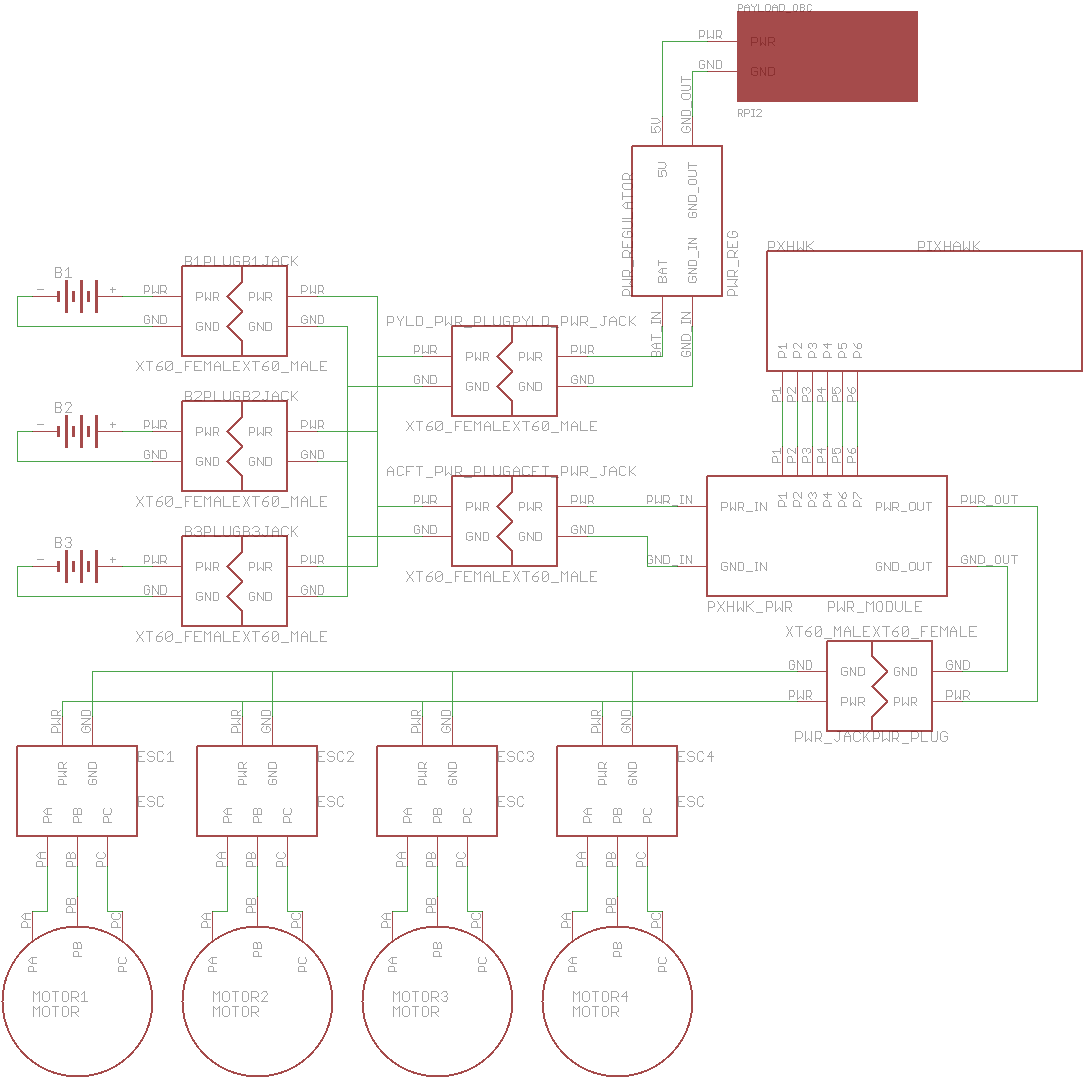
\includegraphics[width=\textwidth]{power_wiring.png}
							\caption{Power Wiring Diagram}
						\end{figure}
				\end{itemize}
			\item Payload Mount \hrulefill CHECK
				\begin{itemize}
					\item Check that the 2 screws are fully threaded and tightened.
					\item Check that the mount is not cracked, twisted, or otherwise damaged.
				\end{itemize}
			\item Payload Wiring\hrulefill CHECK
				\begin{enumerate}
					\item RF IN \dotfill PAYLOAD ANTENNA
					\item DATA STORAGE \dotfill USB PORT
				\end{enumerate}
			\item Payload Antenna\hrulefill CHECK
				\begin{itemize}
					\item Check that the antenna is straight and not touching anything other than where it is mounted on the aircraft.
					\item Check that the antenna is mounted on the insulated part of the boom.
				\end{itemize}
			\item Flight Checks\hrulefill CHECK
				\begin{enumerate}
					\item Power On Check
						\begin{enumerate}
							\item Disconnect the BATTERY PARALLEL ADAPTER from all connections.
							\item Connect the AIRCRAFT BATTERY PACK to the BATTERY PARALLEL ADAPTER.
							\item Connect the BATTERY PARALLEL ADAPTER to AIRCRAFT POWER.
							\item Check that the AUTOPILOT comes online and initializes.
							\item Check that the AUTOPILOT STATUS LIGHT begins to slowly flash within 30 seconds.
							\item Check that the SAFETY SWITCH is blinking red.
							\item Connect the BATTERY PARALLEL ADAPTER to PAYLOAD POWER.
							\item Check that the PAYLOAD STATUS LIGHT immediately begins to quickly flash green.
							\item Disconnect the BATTERY PARALLEL ADAPTER from all connections.
						\end{enumerate}
					\item Avionics Check
						\begin{enumerate}
							\item Disconnect the BATTERY PARALLEL ADAPTER from all connections.
							\item Connect the AIRCRAFT BATTERY PACK to the BATTERY PARALLEL ADAPTER.
							\item Connect the BATTERY PARALLEL ADAPTER to AIRCRAFT POWER.
							\item Check that the AUTOPILOT comes online and initializes.
							\item Check that the AUTOPILOT STATUS LIGHT begins to slowly flash within 30 seconds.
							\item Check that the SAFETY SWITCH is blinking red.
							\item Connect the \gls{gcs} MAVLINK to the AUTOPILOT.
							\item In the \gls{gcs}, check that the GPS satellite count is climbing to at least 6, and that the GPS location is stable and sane.
							\item In the \gls{gcs}, check that the attitude and orientation indicated by the artificial horizon is sane and reacting properly to inputs to the airframe.
							\item In the \gls{gcs}, check that the heading indicated by the compass is sane and reacting properly to inputs to the airframe.
							\item In the \gls{gcs}, check that the AUTOPILOT is receiving commands from the RC TRANSMITTER.
							\item In the \gls{gcs}, check that the battery voltage is sane and agrees with the current battery state.
							\item Connect the BATTERY PARALLEL ADAPTER to PAYLOAD POWER.
							\item Check that the PAYLOAD STATUS LIGHT begins to slowly flash green within 15 seconds.
							\item Disconnect the BATTERY PARALLEL ADAPTER from all connections.
						\end{enumerate}
					\item Spin Up Check
						\begin{enumerate}
							\item Disconnect the BATTERY PARALLEL ADAPTER from all connections.
							\item Connect the AIRCRAFT BATTERY PACK to the BATTERY PARALLEL ADAPTER.
							\item Connect the BATTERY PARALLEL ADAPTER to AIRCRAFT POWER.
							\item Check that the AUTOPILOT comes online and initializes.
							\item Check that the AUTOPILOT STATUS LIGHT begins to slowly flash within 30 seconds.
							\item Check that the SAFETY SWITCH is blinking red.
							\item Check that the RC TRANSMITTER is on and active.
							\item Set the THROTTLE to 0\%.
							\item Set the RC TRANSMITTER MODE SWITCH to STABILIZE.
							\item Disable aircraft safeties by pressing and holding the AIRCRAFT SAFETY SWITCH.
							\item Arm the THROTTLE ARM by holding the left stick down and to the right.
							\item Confirm that the rotors begin spinning in the proper directions.
							\item Advance THROTTLE to 10\%.
							\item Confirm that the right stick inputs are properly executed by the aircraft.
							\item Reduce THROTTLE to 0\%.
							\item Disarm the THROTTLE ARM by holding the left stick down and to the left.
							\item Enable aircraft safeties by pressing and holding the AIRCRAFT SAFETY SWITCH.
							\item Confirm that aircraft safeties are enabled (AIRCRAFT SAFETY SWITCH should be blinking red).
							\item Disconnect the BATTERY PARALLEL ADAPTER from all connections.
						\end{enumerate}
					\item Flight Check
						\begin{enumerate}
							\item Plan a mission with the following parameters:
								\begin{itemize}
									\item Takeoff waypoint immediately above the takeoff area, altitude at least 10 meters AGL.
									\item Waypoint 2 at least 100 meters away, at least 20 meters above takeoff waypoint.
									\item Waypoint 3 at least 100 meters away from previous waypoints, within VLOS, same altitude as Waypoint 2.
									\item Waypoint 4 is a RETURN TO HOME command.
									\item Total flight time is at lest 5 minutes.
								\end{itemize}
							\item Disconnect the BATTERY PARALLEL ADAPTER from all connections.
							\item Connect the AIRCRAFT BATTERY PACK to the BATTERY PARALLEL ADAPTER.
							\item Connect the BATTERY PARALLEL ADAPTER to AIRCRAFT POWER.
							\item Check that the AUTOPILOT comes online and initializes.
							\item Check that the AUTOPILOT STATUS LIGHT begins to slowly flash within 30 seconds.
							\item Check that the SAFETY SWITCH is blinking red.
							\item Check that the RC TRANSMITTER is on and active.
							\item Connect the \gls{gcs} MAVLINK to the AUTOPILOT.
							\item Upload the planned mission.
							\item Conduct the mission with a takeoff in STABILIZE.  Check for abnormal wobbling, uncertain tracking, etc.  All waypoint transitions should be smooth.
							\item Allow aircraft to autoland and manually disarm and safe.
							\item Repeat the mission with a takeoff in LOITER.
						\end{enumerate}
					\item Failsafe Check
						\begin{enumerate}
							\item Plan a mission with the following parameters:
								\begin{itemize}
									\item Takeoff waypoint at least 50 meters AGL.
									\item Waypoint 2 at 100-200 meters distance, 100 meters AGL.
									\item Waypoint 3 at no more than 50 meters distance, at least 20 meters AGL.
									\item Waypoint 4 is a RETURN TO HOME command.
								\end{itemize}
							\item Execute the mission.  When the copter is heading away, turn off the RC TRANSMITTER.  Confirm that the aircraft immediately enters a RETURN TO HOME mode.  Retake control.
							\item Restart the mission.  When the copter is heading away, turn off the \gls{gcs} MAVLINK by turning off the \gls{gcs} AUTOPILOT RADIO.  Confirm that the aircraft immediately enters a RETURN TO HOME mode.  Retake control.
							\item Land and safe the aircraft.
						\end{enumerate}
					\item Payload Check
						\begin{enumerate}
							\item Activate and deploy a known collar at a known location.
							\item Plan a mission starting at least 50 meters away from the known collar that overflies the known collar location.
							\item Run the above mission at an altitude of no more than 30 meters AGL.
							\item Process the data, and confirm that the collar was detected.
						\end{enumerate}
				\end{enumerate}
		\end{enumerate}
	\section{Replacing Propellers}
		Carbon fiber propellers should be replaced if they show signs of cracking or damage.  This manifests as cracks or delamination of the propeller, usually near the tip, but occasionally near the root of the propeller.  To check for cracks or delamination of the propeller, feel along all surfaces of the propeller for any sharp edges or nicks - this is usually the starting point of delamination.  Additionally, flex the propellers to check for any cracking - this will manifest as cracking sounds and the feeling that the propeller is abnormally easier to flex.

		To remove the propeller, remove the two screws and plate holding the propeller to the motor.  Remove the propeller.

		To install the propeller, place the propeller on the rotor shaft, and align the propeller to the screw holes.  Install the top plate and the screws.  Tighten.
	\section{Replacing Arms}
		To remove the arms, first pop the arm to be replaced towards the midline of the copter.  Once the arm is disengaged from plastic keeper, remove the screws holding the boom to the body of the aircraft.  The screw on the top of the body is hidden underneath the autopilot.  Simply push the autopilot gently out of the way to access the screw.  Pull the arm out of the body.  Disconnect the motor power cables.

		To install the arms, first route the motor power cable to the proper side of the arm so that the cables do not get pinched between the arm and the plastic keeper.  Next, insert the arm into the body of the aircraft, and line up the screw holes.  The screw on the top of the body is hidden underneath the autopilot.  Simply push the autopilot gently out of the way to access the screw hole.  Install the screws.  Push the arm towards the plastic keeper until the keeper engages.  Connect the motor power wires.  Conduct the Spin Up Check to ensure that the motor is wired correctly.  If the motor spins backwards, flip any two motor power wires.  Conduct the Propeller Alignment Procedure to properly align the propellers.
	\section{Replacing the Payload Antenna}
		To replace the payload antenna, first disconnect the payload antenna from the payload by unscrewing the SMA connector on the antenna.  Next, uninstall the antenna by removing the zip ties holding the antenna to the copter.

		To install the payload antenna, first check that the insulating tape on the copter booms is intact.  Next, attach the antenna to the copter using zip ties.  Ensure that the antenna is only contacting the insulating tape, and not the carbon fiber booms.  Next, connect the SMA connectors on the antenna and the payload.
	\section{Replacing the Payload}
		To remove the payload, first disconnect the payload power, autopilot telemetry cable, and payload antenna from the payload.  Next, remove the two screws holding the payload to the aircraft.

		To install the payload, align the payload with the existing screw holes on the aircraft so that the user interface devices face the outside of the aircraft.  Install the two screws to secure the payload to the aircraft.  Connect the payload power, autopilot telemetry cable, and payload antenna to the payload.
	\section{Charging Batteries}
		When charging batteries, it is important to ensure that the batteries assigned to a flight pack are charged and discharged together.  This ensures that all the cells are balanced and taking the same amount of wear and tear, reducing the risk of a single cell being depleted and destroying the rest of the cells.

		The first time the batteries are charged, charge all of the batteries individually, then split them into their flight packs.

		For the remaining time that batteries are charged, charge all batteries in their flight packs.

		To charge a single battery, connect the battery's main plug into the charging adapter and insert the battery's balance plug into the charger.  Configure the charger for a maximum current of 5.3 amps, 3 cell LiPo, and a maximum charge of 5500 mAh.

		To charge a complete pack (3 matched batteries), connect each battery's main plug into to the charging adapter and each battery's balance plug into the parallel adapter.  Configure the charger for a maximum current of 16 amps, 3 cell LiPo, and a maximum charge of 16000 mAh.

		To initiate the charging process, press and hold the ``Start'' button until the charger beeps and initiates the ``Battery Check'' sequence.  The charger will then begin the charging process.

		To end the charging process, press the ``Stop'' button.  Verify that the charger has stopped charging, and disconnect the battery's main plug and balance plug.
\chapter{Flight Management Software}
	\section{Requirements}
		\begin{itemize}
			\item Minimum Operating System: Windows 7
			\item Known Good Versions: 1.3.37
		\end{itemize}
	\section{Installation}
		\begin{enumerate}
			\item Download the Mission Planner Installer from http://ardupilot.com
			\item Accept the default settings.
			\item Install the additional drivers when prompted to.
			\item Click finish.
		\end{enumerate}
	\section{Flight Planning}
		\subsection{Selecting a Search Area}
			\begin{enumerate}
				\item Right click to open the context menu.
				\item Under ``Draw Polygon'', select ``Add Polygon Point''.
				\item Click ``OK''.
				\item Drag the first point to the desired location.
				\item Click to set additional points.
			\end{enumerate}
		\subsection{Loading a Search Area}
			\begin{enumerate}
				\item Right click to open the context menu.
				\item Under ``Draw Polygon'', select ``Load Polygon''.
				\item Select the polygon file you wish to load.
			\end{enumerate}
		\subsection{Saving a Search Area}
			\begin{enumerate}
				\item Right click to open the context menu.
				\item Under ``Draw Polygon'', select ``Save Polygon''.
				\item Enter the filename and directory in which you would like to save the polygon file.
				\item Click ``Save''.
			\end{enumerate}
		\subsection{Plotting a Search Grid}
			\begin{enumerate}
				\item Set a search area.
				\item Right click to open the context menu.
				\item Under ``Auto WP'', select ``Survey (Grid)''.
				\item Check the ``Advanced Options'' checkbox under ``Display'' on the right-hand sidebar.
				\item Set the desired altitude and flight speed.
				\item Check the ``Add Takeoff and Land WP's'' and ``Use \gls{rtl}'' checkboxes.
				\item Open the ``Grid Options'' tab.
				\item Set the ``Distance between lines [m]'' to 30 meters.
				\item Check that the ``Flight Time (est)'' field on the bottom bar is less than 20 minutes.
				\item Click ``Accept''.
				\item Check that the waypoints have been properly set.
			\end{enumerate}
		\subsection{Saving a Mission}
			\begin{enumerate}
				\item Click the ``Save WPs'' button in the right-hand sidebar.
				\item Select the desired directory and filename and save.
			\end{enumerate}
		\subsection{Opening a Saved Mission}
			\begin{enumerate}
				\item Click the ``Load WPs'' button in the right-hand sidebar.
				\item Navigate to the desired waypoints file and click ``Open''.
				\item Click ``OK'' when prompted to replace the HOME location.
			\end{enumerate}
	\section{Uploading a Mission}
		\begin{enumerate}
			\item Load a mission into Mission Planner.
			\item Connect to the \gls{uas} with MAVLINK.
			\item Click the ``Write WPs'' button on the right-hand sidebar.
			\item Click the ``Read WPs'' button on the right-hand sidebar.
			\item Click ``OK'' to the dialog prompting you to reset the HOME location.
			\item Verify that the waypoints now displayed are the desired mission waypoints.
		\end{enumerate}
	\section{Operating a Mission}
		The primary responsiblity of the \gls{AO} is to monitor the \gls{uas} as it progresses through its programmed mission.  During this time, the autopilot operator should be monitoring the vital signs from the \gls{uas}, including ground speed, mission progress, altitude, attitude, stability, battery voltage, battery consumption, power draw, and navigation stability, among other things.  In most cases, monitoring the artificial horizon and flight map will suffice - check that the \gls{uas} is tracking properly to the waypoints, and that the airctaft has a reasonable attitude for its current speed and heading.  Occasionally, check the battery voltage and consumption to ensure that the \gls{uas} has enough power to complete the mission and return.
\printglossary[type=main,nonumberlist]
\end{document}
